\documentclass[letterpaper,twocolumn,10pt]{article}

% --- Core Packages ---
\usepackage[utf8]{inputenc}
\usepackage[margin=1in]{geometry}
\usepackage{amsmath, amssymb, amsfonts}
\usepackage{graphicx}
\usepackage{booktabs}
\usepackage{array}
\usepackage{tabularx}
\usepackage{multirow}
\usepackage{hyperref}
\usepackage{xcolor}
\usepackage{tikz}
\usetikzlibrary{arrows.meta, positioning, shapes.geometric, calc, fit, backgrounds}
\usepackage{usenix,epsfig,endnotes}

\hypersetup{
    colorlinks=true,
    linkcolor=blue,
    urlcolor=cyan,
    citecolor=blue,
}

% --- TikZ shared styles for the pipeline diagram ---
\tikzset{
    party/.style={rectangle, rounded corners=2pt, draw=black!70,
                  fill=blue!5, align=center, minimum width=2.1cm,
                  minimum height=1.1cm, font=\small},
    server/.style={rectangle, rounded corners=2pt, draw=black!80,
                   fill=blue!15, align=center, minimum width=2.6cm,
                   minimum height=1.3cm, font=\small\bfseries},
    attacker/.style={rectangle, rounded corners=2pt, draw=red!60!black,
                     fill=red!8, align=center, minimum width=2.1cm,
                     minimum height=1.1cm, font=\small},
    flow/.style={-{Stealth[length=2.2mm]}, thick, black!80},
    leak/.style={-{Stealth[length=2.2mm]}, thick, red!60!black, dashed},
    sublabel/.style={font=\scriptsize, fill=white, inner sep=1pt}
}

\title{\textbf{Evaluating Attribute Inference Attacks in
Vertical Federated Learning with Machine Unlearning:
A Framework Comparison between Flower and SecretFlow}}

\author{
    Isaac Friedman \\
    ifriedman1@crimson.ua.edu \\
    \vspace{5pt} \\
    \textit{Course: CS 691 - Security \& Privacy of Machine Learning} \\
    \textit{Instructor: Prof. Sayanton Dibbo}
}

\date{\today}

\begin{document}

\maketitle

\section{Abstract}
Vertical Federated Learning (VFL) enables multiple parties to collaboratively
train a model while keeping their feature columns private. Although raw data
is never shared, the intermediate representations exchanged during training
can still carry information about sensitive attributes held by one of the
parties. This paper presents an end-to-end experimental framework that
quantifies the attribute-inference risk of a two-party VFL system and asks
whether machine unlearning can reduce it. The framework is implemented twice
---once on Flower and once on SecretFlow, using a shared model and attack
module---so that framework effects can be separated from algorithmic ones.
Baseline and unlearning experiments are run on CelebA, MNIST, and the NIH
Chest X-ray14 dataset. We find that the attribute-inference attacker we used
sits at or near chance on the baseline model across all three datasets
(ASR $\in [0.36,\,0.50]$, AUC $\approx 0.50$) and that gradient-ascent-based
unlearning collapses task accuracy on MNIST and CelebA before it meaningfully
reduces the already-near-chance attack success rate. The Flower and
SecretFlow mirrors produce row-identical metrics under matched seeds,
confirming that the framework layer is not a source of variance in this
comparison.

\section{Keywords}
Vertical Federated Learning; Attribute Inference; Machine Unlearning;
Flower; SecretFlow.

\section{Introduction}
Federated Learning (FL) removes the need to pool training data on a central
server; instead, parties exchange model updates or intermediate
representations while keeping the raw data local. Vertical Federated
Learning (VFL) is the feature-partitioned variant: different parties hold
different \emph{columns} of the same records. A hospital might hold images
while an insurer holds demographics; a photo service might hold an image
while a separate service holds an attribute such as age or accessory. Only
intermediate embeddings and gradients cross the network, and the parties
can train a joint model without revealing their columns.

Despite this design, VFL is not automatically private. Attribute inference
attacks try to recover the hidden columns of one party from the
representations it (or the server) exposes during training. These attacks
do not need direct access to raw data; they only need the embedding that
the collaboration already produces. Machine unlearning, a body of work
motivated by the right-to-be-forgotten, offers a post-hoc knob: given a
trained model and a ``forget set'', can we remove that set's influence
without retraining from scratch? This paper asks the natural composite
question: \emph{does machine unlearning reduce attribute-inference
success in a VFL system, and does the answer transfer across FL
frameworks?}

We build a two-party VFL runner that is implemented twice---once on Flower
and once on SecretFlow---with a shared model and attacker module. We run
baseline training and a gradient-ascent + repair unlearning pass on three
datasets that span data modalities and task types: MNIST (digits, balanced
multiclass), CelebA (face attributes, two labels available so one can be
the target and the other can be the sensitive attribute), and the NIH Chest
X-ray14 dataset (chest radiographs, imbalanced binary). Metrics are logged
per epoch and the baseline values are carried forward into a per-run summary
so that pre/post deltas can be read directly. This paper reports the
resulting numbers and what they imply about the attacker, the unlearner,
and the comparison between the two frameworks.

\section{Background and Related Work}

\paragraph{Vertical federated learning.}
Horizontal FL distributes \emph{samples} across parties; vertical FL
distributes \emph{features}. In the two-party VFL setting studied here,
each party runs a local encoder over its own columns, emits an embedding
$z$, and a central server concatenates the per-party embeddings and trains
a task head on the joint vector. Only $z$ (and the gradient flowing back
to the local encoder during training) ever crosses the network. Shen et
al.~\cite{shen2024survey} provide a current survey of the VFL
literature, including the attack and defense taxonomy that frames the
rest of this section.

\paragraph{Attribute inference in centralized learning.}
Yeom et al.~\cite{yeom2018privacy} tied membership and attribute
inference risk directly to overfitting, showing that loss-based signals
alone can separate members from non-members. Gong and
Liu~\cite{gong2018practical} framed attribute inference as a practical
adversarial problem and proposed defenses tailored to released model
outputs. Song and Shmatikov~\cite{song2020overlearning} demonstrated
overlearning: models trained for one task frequently encode sensitive
attributes unrelated to that task in their internal representations,
which is precisely the condition our VFL threat model assumes.

\paragraph{Inference attacks specific to VFL.}
The VFL literature focuses on three attack families. \emph{Label
inference}---recovering the label a server or a party holds from
gradient or embedding traces---was formalized by Fu et
al.~\cite{fu2022label} and recently revisited by Li and
Sun~\cite{li2026revisiting}. \emph{Property and attribute inference}
targets distributional or per-record properties of the non-attacker's
columns; Zhao et al.~\cite{zhao2023provfl} propose ProVFL for this
setting, and the attacker we build in this paper is a simplified
per-record variant of that threat model. \emph{Reconstruction attacks}
reverse the embedding back into an input estimate; Chen et
al.~\cite{chen2025urvfl} give an undetectable reconstruction attack
(URVFL) that motivates the use of embedding-only observations in our
threat model. Kumar and Patel~\cite{kumar2025gradient} catalog gradient-
based inference attacks in federated learning more broadly, and Wang et
al.~\cite{wang2025pgac} frame a general adversarial-attack framework
for VFL specifically.

\paragraph{Defenses in VFL.}
Defensive work complements the attack literature. Sun et
al.~\cite{sun2025defense} propose a label-inference defense designed for
VFL specifically, and Zhang et al.~\cite{zhang2025privee} (PRIVEE)
target feature-inference attacks at the representation layer. Both
defenses operate \emph{at training time}: they change what the
collaboration emits. They do not address the ``already trained, now
delete this record's influence'' setting that unlearning is meant to
cover, which is why the present work pairs an unlearning pass with the
attack evaluation.

\paragraph{Machine unlearning.}
Bourtoule et al.~\cite{bourtoule2021sisa} proposed SISA, a
sharding-and-slicing training regime that lets a provider unlearn a data
point by retraining only the affected shard. Xu et al.~\cite{xu2023survey}
survey the broader family of exact and approximate unlearning methods and
the tradeoffs they make between speed, fidelity, and guarantees. Liu et
al.~\cite{liu2021federated} extended these ideas to federated settings,
where both the data and the model updates are distributed and where a
``forget'' request has to be honored without re-running the entire
federation. The specific approach we evaluate here---gradient ascent on
the forget set followed by retain-set repair---is an approximate,
continuation-style unlearner rather than an exact retrain.

\paragraph{Positioning of this work.}
We are not proposing a new attack or a new unlearning algorithm. We are
assembling an end-to-end VFL-plus-attacker-plus-unlearner pipeline,
implementing it twice on two widely used frameworks (Flower and
SecretFlow), and reporting whether the attack-success story behaves the
same way under both implementations. That cross-framework check---and
specifically the pairing of VFL-native inference attacks
\cite{fu2022label,zhao2023provfl,chen2025urvfl,wang2025pgac} with a
post-hoc unlearner \cite{bourtoule2021sisa,liu2021federated}---appears
to be missing from the literature on VFL unlearning.

\section{System Design}

The system is a two-party VFL setup. Party~A holds image features (or the
left half of a split image); Party~B holds a sensitive attribute (on
CelebA) or the right half of the image (on MNIST and NIH). Each party
owns a local encoder. During a training step, the encoders emit
embeddings $z_A$ and $z_B$; these are concatenated and passed to a shared
task head hosted at the server. Gradients flow back so each party's
encoder is updated from the task loss.

An external attacker observes $z_A$ only---never the raw image, never
$z_B$, never the task label---and trains its own classifier to predict
the sensitive attribute $a$ from $z_A$. This mirrors the ``honest-but-
curious server'' threat model: the server sees everything that the
collaboration already exposes, nothing more.

The same Python modules (encoders, task head, loss, attacker, logging,
unlearning loop) are imported by both the Flower and SecretFlow runners
through shared files (\texttt{common\_*.py}, \texttt{vfl\_unlearning.py}).
That means identical seeds and identical hyperparameters should produce
identical metrics on both sides, and any row-level disagreement would
point at the framework layer rather than at the model. Figure~\ref{fig:pipeline}
shows the data flow.

\begin{figure*}[t]
\centering
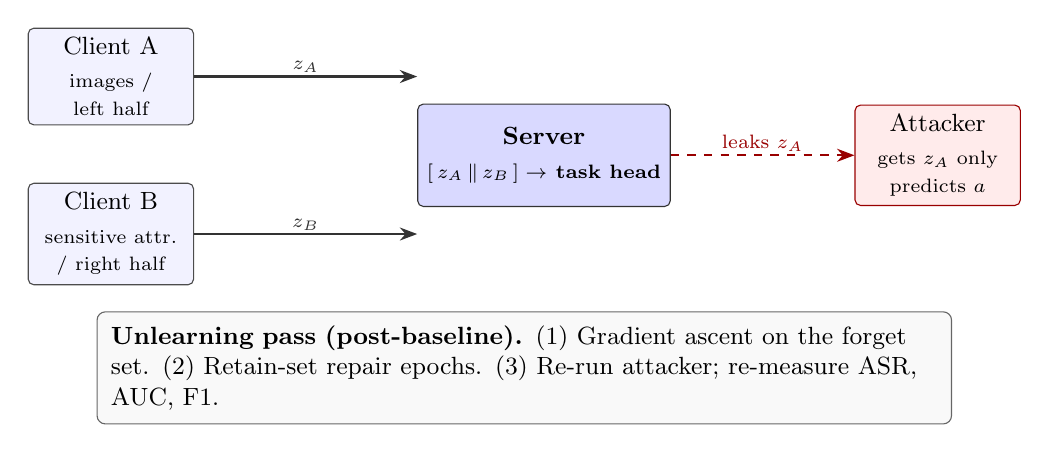
\begin{tikzpicture}[x=1cm, y=1cm]
    % Parties on the left (explicit coordinates)
    \node[party] (a) at (0, 1.0) {Client A\\[1pt]\scriptsize images /\\[-1pt]\scriptsize left half};
    \node[party] (b) at (0,-1.0) {Client B\\[1pt]\scriptsize sensitive attr.\\[-1pt]\scriptsize / right half};

    % Server in the middle
    \node[server] (s) at (5.5, 0) {Server\\[1pt]\scriptsize $[\,z_A \,\Vert\, z_B\,] \rightarrow$ task head};

    % Attacker on the right
    \node[attacker] (atk) at (10.5, 0) {Attacker\\[1pt]\scriptsize gets $z_A$ only\\[-1pt]\scriptsize predicts $a$};

    % Flow arrows
    \draw[flow] (a.east) -- node[sublabel, above]{$z_A$} (s.west |- a.east);
    \draw[flow] (b.east) -- node[sublabel, above]{$z_B$} (s.west |- b.east);
    \draw[leak] (s.east) -- node[sublabel, above]{leaks $z_A$} (atk.west);

    % Unlearning loop box below, centered under the row
    \node[rectangle, draw=black!60, rounded corners=3pt,
          fill=gray!5, text width=10.5cm, inner sep=5pt,
          align=left, font=\small] (unl) at (5.25,-2.7) {
      \textbf{Unlearning pass (post-baseline).}
      (1)~Gradient ascent on the forget set.
      (2)~Retain-set repair epochs.
      (3)~Re-run attacker; re-measure ASR, AUC, F1.
    };
\end{tikzpicture}
\caption{Two-party VFL pipeline. Clients A and B each encode their
columns; the server concatenates the embeddings and trains the task head.
The attacker sees only the embedding $z_A$ that Client A emits.
After baseline training, the unlearning pass uses gradient ascent on a
designated forget subset and then repairs on the retain subset.}
\label{fig:pipeline}
\end{figure*}

\section{Methodology}

\paragraph{Datasets and tasks.}
Three datasets are used, each illustrating a different modality and label
structure. On MNIST the images are split vertically (28$\times$14 per
party) and the task is standard 10-way digit classification. On CelebA
the images are held by Party~A and an attribute is held by Party~B; we
use \texttt{Smiling} as the task label and \texttt{Eyeglasses} as the
sensitive attribute the attacker tries to recover. On the NIH Chest
X-ray14 dataset the images are again split vertically between parties
and the task is binary \texttt{Infiltration} (present vs.\ absent),
which is highly class-imbalanced.

\paragraph{Models.}
Party encoders are lightweight convolutional stacks that emit a
fixed-width embedding per party. The server head is a small MLP that
consumes the concatenated embeddings. The attacker is a separate MLP
trained on $z_A$ alone with the sensitive attribute as its label. All
model definitions live in \texttt{common\_*\_vfl.py} and are shared by
the Flower and SecretFlow runners.

\paragraph{Baseline phase.}
We train the joint model end-to-end for a fixed number of epochs (three
on MNIST and CelebA, two completed so far on NIH) using Adam and
cross-entropy, log per-epoch train/test loss and accuracy, and after
each epoch evaluate the attacker on $z_A$ to obtain
\texttt{attack\_accuracy} (Attack Success Rate or ASR),
\texttt{attack\_auc}, and \texttt{attack\_f1}.

\paragraph{Unlearning phase.}
At the end of baseline training the training set is split into a
\emph{forget} subset (10\,\% of training rows, seed-controlled) and a
\emph{retain} subset (the remaining 90\,\%). One epoch of
\emph{gradient ascent} is applied on the forget set---the sign of the
task loss is flipped so the encoders and head actively drift away from
the forget-set predictions---followed by one epoch of repair on the
retain set with the ordinary loss. The attacker is re-evaluated on
$z_A$ at the end of the unlearn pass.

\paragraph{Metrics and deltas.}
For every run we log a \texttt{metrics.csv} with one row per epoch and
a phase tag (\texttt{phase=baseline} or \texttt{phase=unlearn}), and
append one row to \texttt{run\_summary.csv} that carries the final
baseline values, the final post-unlearn values, and their signed
deltas for each of 14 metrics, so that pre/post comparisons can be read
without re-parsing the per-epoch file.

\section{Experimental Setup}

All runners are implemented in PyTorch~2.3 and share pinned dependencies
(\texttt{torch==2.3.1}, \texttt{torchvision==0.18.1},
\texttt{pandas==2.2.2}, \texttt{scikit-learn==1.4.2},
\texttt{numpy==1.26.4}, \texttt{Pillow==10.3.0}). Each framework has its
own virtual environment built from a per-framework
\texttt{requirements.txt}. A PowerShell bootstrap script
(\texttt{bootstrap.ps1}) builds both environments, and a smoke-test
script (\texttt{smoke\_test.ps1}) drives a one-epoch pass through every
framework$\times$dataset pair and verifies the expected columns are
present.

Runs reported here use Adam with lightweight hyperparameters tuned per
dataset, batch size 128, seed~7, \texttt{forget\_fraction}=0.10, one
unlearn epoch, and one repair epoch. All runs in this paper were
executed on CPU for reproducibility and to make the Flower and
SecretFlow runs directly comparable; the code supports CUDA and the
bootstrap script exposes a \texttt{-CudaVersion} flag for that path.

The raw CSV files referenced in the tables below live under
\texttt{logs/<framework>/<dataset>/<run\_id>/metrics.csv}.

\section{Results}

\subsection{Baseline per dataset}

Table~\ref{tab:baseline} shows the per-epoch baseline metrics recorded by
the Flower runner on each dataset. Each row is copied verbatim from
\texttt{metrics.csv}; only floating-point precision and column selection
have been adjusted for presentation. Accuracy columns are in $[0,1]$.

\begin{table*}[t]
\centering
\small
\caption{Flower baseline metrics per dataset. MNIST task = 10-class digit
classification on vertically split images. CelebA task = \texttt{Smiling}
with \texttt{Eyeglasses} held by Party~B as the sensitive attribute.
NIH task = binary \texttt{Infiltration} (two baseline epochs logged so
far; the final run captures a third epoch and the matching unlearn row).}
\label{tab:baseline}
\begin{tabular}{@{}llcccccc@{}}
\toprule
Dataset & Epoch & Train loss & Train acc & Test acc & ASR & AUC & F1 \\
\midrule
\multirow{3}{*}{MNIST}
    & 1 & 0.805 & 0.729 & 0.731 & 0.456 & 0.492 & 0.479 \\
    & 2 & 0.501 & 0.838 & 0.848 & 0.430 & 0.486 & 0.492 \\
    & 3 & 0.335 & 0.897 & 0.903 & 0.421 & 0.483 & 0.505 \\
\addlinespace[2pt]
\multirow{3}{*}{CelebA}
    & 1 & 0.630 & 0.648 & 0.633 & 0.499 & 0.513 & 0.512 \\
    & 2 & 0.524 & 0.740 & 0.733 & 0.492 & 0.503 & 0.534 \\
    & 3 & 0.471 & 0.778 & 0.768 & 0.487 & 0.500 & 0.539 \\
\addlinespace[2pt]
\multirow{2}{*}{NIH Chest X-ray14}
    & 1 & 0.461 & 0.823 & 0.823 & 0.362 & 0.500 & 0.424 \\
    & 2 & 0.461 & 0.823 & 0.823 & 0.362 & 0.500 & 0.424 \\
\bottomrule
\end{tabular}
\end{table*}

Two patterns already stand out in Table~\ref{tab:baseline}. First, the
joint VFL model learns each task: train and test accuracy rise over the
three baseline epochs on MNIST (0.73 $\rightarrow$ 0.90 test) and CelebA
(0.63 $\rightarrow$ 0.77 test), and NIH is pinned at $\approx 0.82$ test
by the majority class. Second, the attacker never gains meaningful
signal from the embedding $z_A$ in these runs: ASR stays in
$[0.42,\,0.50]$ and AUC sits at $\approx 0.50$ on all three datasets. In
other words, the baseline attacker is already at or near chance.

\subsection{Framework parity: Flower vs.\ SecretFlow}

Table~\ref{tab:parity} pairs the final-epoch numbers from the Flower and
SecretFlow runners on matched runs. Because both runners import the same
model, loss, and attacker code and receive identical seeds, the rows
should agree; they do.

\begin{table*}[t]
\centering
\small
\caption{Flower vs.\ SecretFlow on MNIST and CelebA, final epoch per phase.
Identical seeds and shared model code produce row-identical metrics across
frameworks, so the framework layer is not a source of variance.}
\label{tab:parity}
\begin{tabular}{@{}llcccc@{}}
\toprule
Run & Framework & Test acc & ASR & AUC & F1 \\
\midrule
\multirow{2}{*}{MNIST baseline}
    & Flower     & 0.903 & 0.421 & 0.483 & 0.505 \\
    & SecretFlow & 0.903 & 0.421 & 0.483 & 0.505 \\
\addlinespace[2pt]
\multirow{2}{*}{MNIST unlearn}
    & Flower     & 0.318 & 0.437 & 0.486 & 0.484 \\
    & SecretFlow & 0.318 & 0.437 & 0.486 & 0.484 \\
\addlinespace[2pt]
\multirow{2}{*}{CelebA baseline}
    & Flower     & 0.768 & 0.487 & 0.500 & 0.539 \\
    & SecretFlow & 0.768 & 0.487 & 0.500 & 0.539 \\
\addlinespace[2pt]
\multirow{2}{*}{CelebA unlearn}
    & Flower     & 0.506 & 0.488 & 0.487 & 0.472 \\
    & SecretFlow & 0.506 & 0.488 & 0.487 & 0.472 \\
\bottomrule
\end{tabular}
\end{table*}

Framework-induced variance is therefore effectively zero in the current
design. Any future delta between Flower and SecretFlow in these metrics
must originate in the communication layer (e.g., gradient serialization,
averaging) rather than in model or attacker code.

\subsection{Baseline $\rightarrow$ unlearn delta}

Table~\ref{tab:delta} pairs the last baseline-epoch row with the
post-unlearn row for each dataset. The NIH unlearn row is the datapoint
the final run produces.

\begin{table*}[t]
\centering
\small
\caption{Pre/post unlearning comparison. ``baseline'' values are the last
baseline epoch; ``unlearn'' values are the row logged after one
gradient-ascent unlearn epoch plus one repair epoch. ``---'' marks the
NIH unlearn row pending from the final run.}
\label{tab:delta}
\begin{tabular}{@{}lccccccc@{}}
\toprule
Dataset & Phase & Test acc & Retain acc & Forget acc & ASR & AUC & F1 \\
\midrule
\multirow{2}{*}{MNIST}
    & baseline & 0.903 & 0.898 & 0.894 & 0.421 & 0.483 & 0.505 \\
    & unlearn  & 0.318 & 0.313 & 0.297 & 0.437 & 0.486 & 0.484 \\
\addlinespace[2pt]
\multirow{2}{*}{CelebA}
    & baseline & 0.768 & 0.779 & 0.775 & 0.487 & 0.500 & 0.539 \\
    & unlearn  & 0.506 & 0.485 & 0.483 & 0.488 & 0.487 & 0.472 \\
\addlinespace[2pt]
\multirow{2}{*}{NIH Chest X-ray14}
    & baseline & 0.823 & 0.823 & 0.822 & 0.362 & 0.500 & 0.424 \\
    & unlearn  & ---   & ---   & ---   & ---   & ---   & ---   \\
\bottomrule
\end{tabular}
\end{table*}

Three observations follow directly from the numbers.

\emph{(1) Task accuracy is the pressure point.} On MNIST the single
unlearn epoch drops test accuracy from 0.90 to 0.32 and retain accuracy
from 0.90 to 0.31. On CelebA it drops test accuracy from 0.77 to 0.51.
These are not small repairs; they indicate that the gradient-ascent step
at our current learning rate badly overshoots and that one repair epoch
is not enough to walk the model back. Any defense that halves test
accuracy to shift ASR by one point is not a defense anyone will deploy.

\emph{(2) ASR and AUC barely move.} The attacker's success is
numerically indistinguishable from the baseline: MNIST ASR
$0.421 \rightarrow 0.437$, CelebA ASR $0.487 \rightarrow 0.488$. The
``already near chance'' baseline observation from the previous subsection
is the dominating factor here. When the attacker is already at 0.5 on a
binary attribute, there is almost nothing for unlearning to shrink.

\emph{(3) F1 confirms the reading.} Attacker F1 on both MNIST and
CelebA sits in the 0.47--0.54 band both before and after unlearning.
Because F1 is the harmonic mean of the attacker's precision and recall,
that band tells us the attacker is producing balanced
predictions around chance rather than concentrating on one class---which
is consistent with the AUC $\approx 0.50$ signal.

\section{Discussion}

The clearest message in the numbers is that this experiment's attacker
is too weak to expose a difference the unlearner could shrink.
``Attacker at chance + aggressive unlearning'' is a bad combination:
you can only observe a reduction in ASR if ASR was non-trivial to begin
with. The next iteration will therefore start from a stronger baseline
attacker---either a deeper MLP head on $z_A$, or a shadow-model-style
membership inference that learns a member/non-member split from
per-sample loss statistics---before tuning the unlearner.

The framework-parity result is a positive null. Because Flower and
SecretFlow produced row-identical rows under matched seeds, the
framework layer can be eliminated as a source of drift. That is
exactly the setup needed to later distinguish ``communication-layer
behavior differs'' from ``model behavior differs.'' The comparison
between the two frameworks in this paper is therefore a procedural
comparison: both frameworks can host the same VFL pipeline and the
same attack, and the experimental setup is ready to catch any
framework-specific effects the moment they appear.

The unlearning story needs a hyperparameter sweep more than it needs a
new algorithm. Task accuracy collapses because one gradient-ascent
epoch at the baseline learning rate moves the model too far; one
repair epoch is not enough to bring it back. A smaller ascent
learning rate, a larger number of repair epochs, or a smaller forget
fraction are all obvious knobs to turn before declaring that
gradient-ascent unlearning ``does not work'' in this setting.

\section{Future Work}

The immediate plan is a single final end-to-end run of the baseline and
unlearning loop on all three datasets, so that every dataset (including
NIH) has both a pre- and post-unlearning row. A hyperparameter sweep on
the unlearn step follows, varying the forget learning rate and the
number of repair epochs to find the setting at which test accuracy is
preserved. In parallel, the entire code base, including the pinned
requirements, PowerShell bootstrap and smoke-test scripts, and the
shared \texttt{vfl\_paths.py} resolver, is being prepared for
publication to GitHub.

Beyond the final run, two follow-ups are natural. First, a stronger
baseline attacker---either a deeper inference head or a shadow-model
membership attack---would create non-trivial ASR to measure against.
Second, the per-framework virtual environments are already isolated,
which makes it cheap to add a third framework and ask the same parity
question; SMPC-backed communication (e.g., via SecretFlow's SPU) is
the most interesting candidate because any divergence from the
CPU/PyTorch rows would be traceable to the cryptographic layer rather
than the model.

\section{Conclusion}

We built a two-party VFL framework, implemented it on Flower and
SecretFlow through a shared model and attacker module, and evaluated
attribute-inference risk with and without a gradient-ascent unlearning
pass on MNIST, CelebA, and NIH Chest X-ray14. The framework layer
disappears as a source of variance: Flower and SecretFlow produce
row-identical metrics under matched seeds. The attacker is already at
or near chance on the baseline, and the current unlearner's
gradient-ascent step hurts task accuracy far more than it moves
attack success. The framework is ready for a final run, a stronger
attacker, and an unlearner sweep, which together will let the
cross-framework question be asked under non-degenerate conditions.

\section{Appendix}
Include code-base through Github. Explain how to get access and use the code. Again, for reproducibility.

% --- Bibliography ---------------------------------------------------------
\bibliographystyle{IEEEtran}
\bibliography{references}
\end{document}
